
\documentclass{beamer}

\usepackage{algpseudocode, color, colortbl}

\usepackage{hyperref}
\hypersetup{
    colorlinks=true,
    urlcolor=blue,
}

\usepackage{tikz, xcolor}

\usetheme{Montpellier}
\usecolortheme{rose}

% page numbers, from
% https://tex.stackexchange.com/questions/137022/how-to-insert-page-number-in-beamer-navigation-symbols
\expandafter\def\expandafter\insertshorttitle\expandafter{%
  \insertshorttitle\hfill%
  \insertframenumber\,/\,\inserttotalframenumber}

\definecolor{Gray}{gray}{0.8}
\newcolumntype{g}{>{\columncolor{Gray}}c}

\newcommand{\stanza}{ \\~\ }

\title{10. The Linear Programming Problem}
\subtitle{CPSC 535 $\sim$ Fall 2019}
\author{Kevin A. Wortman}
\institute{ 
\includegraphics[height=2cm]{csuf-logo-cmyk} }
\date{October 28, 2019 \stanza

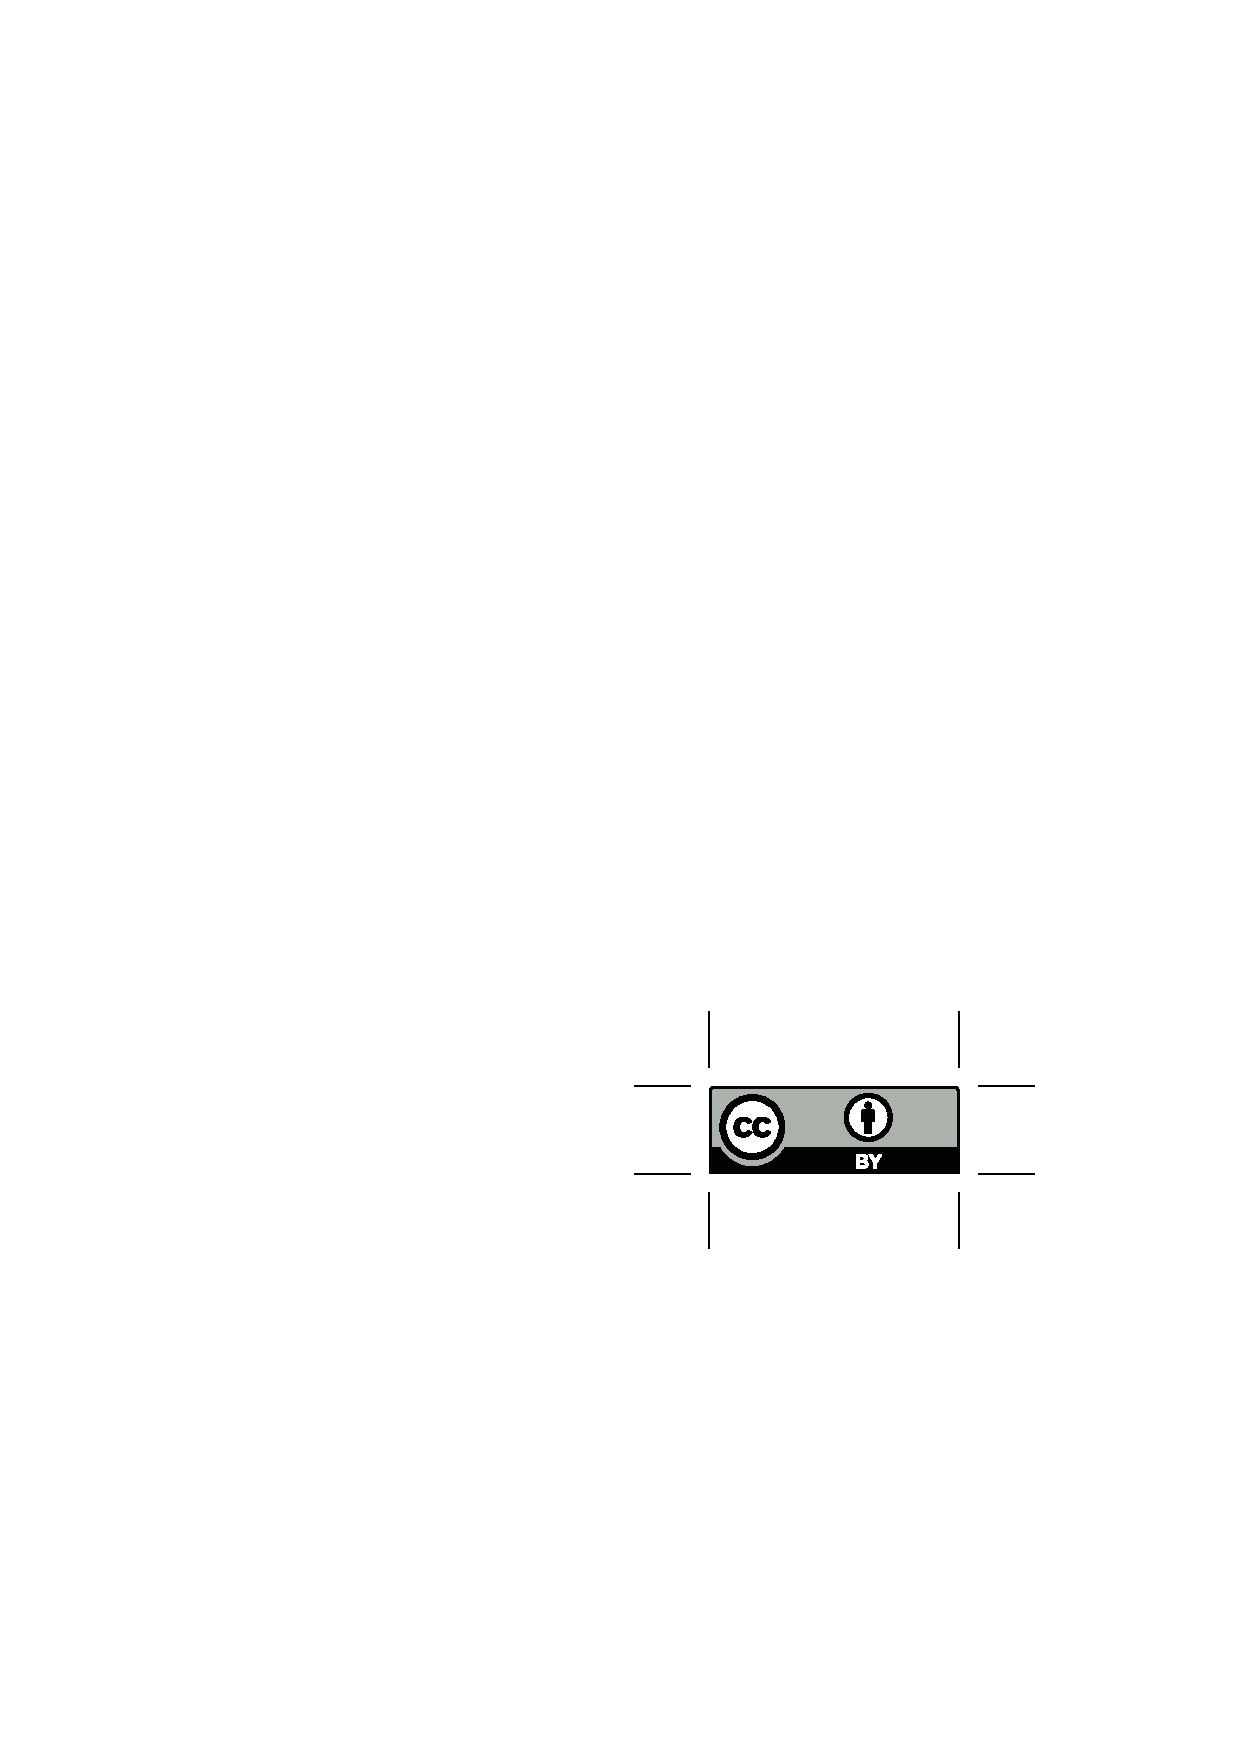
\includegraphics[height=14pt]{by} \\

{\tiny
This work is licensed under a
\href{http://creativecommons.org/licenses/by/4.0/}{Creative Commons Attribution 4.0 International License}.
}}

\begin{document}

\begin{frame}
  \titlepage
\end{frame}

\begin{frame} \frametitle{Big Ideas}
\begin{itemize}
  \item duality --- same problem from different perspectives
  \item formulations, reductions
  \item visualizing high geometric dimensions
\end{itemize}
\end{frame}

\begin{frame} \frametitle{Overview}
  \begin{itemize}
    \item \emph{programming} in math involves finding some kind of optimal solution
      subject to mathematically-codified constraints
      \begin{itemize}
        \item (not coding e.g. C++ programming)
      \end{itemize}
    \item \emph{linear programming (LP):} optimize a linear \emph{objective function}
      subject to inequalities
    \item very general framework
    \item pioneered by Soviet economist Leonid Kantorovich circa 1930s; goal
      was to optimize supply/demand in a communist in lieu of prices
    \item now used in business \emph{(operations research)}
    \begin{itemize}
      \item scheduling UPS deliveries, optimizing farm production, allocating
        investment portfolios, etc.
    \end{itemize}
  \end{itemize}
\end{frame}

\begin{frame} \frametitle{Computational Complexity}
  \begin{itemize}
    \item many tough problems in $P$, including max-flow, reduce to LP
    \item on the border of $P$
    \item simplex algorithm technically takes $O(2^n)$ worst-case time,
      but is fast polynomial on most practical inputs
    \item we have pseudopolynomial algorithms with e.g. $O(n^{2.5} W)$ runtime
      and expensive constant factors
    \item open question whether there is a strongly polynomial LP algorithm with runtime
      e.g. $O(n^3),$ not a function of $W$
  \end{itemize}
\end{frame}

\begin{frame} \frametitle{Standard Form}
\begin{itemize}
  \item \emph{standard form:} restricted/simplified LP, easier for algorithms to solve
  \item later: \emph{general form} which is more convenient for end-user
    formulations
  \item general reduces to standard with constant overhead
  \item similar situation to max-flow and robust max-flow
  \item actual solver algorithm sees a simplified standard form; reduction
    algorithm ``frontend'' accepts a generalized problem that is more convenient
    for end-users
\end{itemize}
\end{frame}

\begin{frame} \frametitle{Standard Form}
standard form with $n$ variables and $m$ constraints:\stanza

maximize $c_1 x_1 + c_2 x_2 + \ldots + c_n x_n$ \\
subject to
\begin{eqnarray*}
a_{1,1} x_1 + a_{1,2} x_2 + \ldots + a_{1, n} x_{1, n} &\leq& b_1 \\
a_{2,1} x_1 + a_{2,2} x_2 + \ldots + a_{2, n} x_{2, n} &\leq& b_2 \\
\vdots & & \vdots \\
a_{m,1} x_1 + a_{m,2} x_2 + \ldots + a_{m, n} x_{m, n} &\leq& b_m \\
x_1, x_2, \ldots, x_n &\geq& 0
\end{eqnarray*}

\emph{variables:} $x_1, \ldots, x_n \in \mathbb{R}$ \\
\emph{objective function} defined by coefficients $c_1, \ldots, c_n \in \mathbb{R}$ \\
\emph{constraints} defined by coefficients $a_{i,j}, b_i \in \mathbb{R}$
\end{frame}

\begin{frame} \frametitle{Standard Form Example}
maximize $2 x_1 + x_2 - \frac{1}{3} x_3$ \\
subject to
\begin{eqnarray*}
x_1 + x_2 &\leq& 10 \\
-x_3 &\leq& -2 \\
x_1, x_2, x_3 &\geq& 0
\end{eqnarray*}
\end{frame}

\begin{frame} \frametitle{Standard Form Matrix Notation}
\begin{itemize}
  \item more compact math notation
  \item collect:
  \begin{itemize}
    \item variables into vector $x=\langle x_1, \ldots, x_n \rangle$
    \item objective coefficients into vector $c=\langle c_1, \ldots, c_n\rangle$
    \item r.h.s. of inequalities into vector $b=\langle b_1, \ldots, b_m\rangle$
    \item $a_{i,j}$ coefficients into matrix $A$
  \end{itemize}
  \item LP can be written in terms of dot-product and matrix-vector multiplication
    as (and note the transpose $c^T$):
\end{itemize}
\vspace{.5cm}
maximize $c^T x$ \\
subject to
\begin{eqnarray*}
  Ax &\leq& b \\
  x &\geq& 0
\end{eqnarray*}
\end{frame}

\begin{frame} \frametitle{Possible Outcomes}
LPs are not always solvable! \stanza

there are three outcomes:
\begin{enumerate}
  \item \textbf{solution}: concrete values for $x_1, \ldots, x_n$ that maximize
    $c^T x$ (good, usually the goal)
  \item \textbf{unbounded}: objective can be made arbitrarily large i.e.
    $+\infty$ (bad, usually means there is a bug in your LP that makes it nonsensical)
  \item \textbf{infeasible}: impossible to satisfy all constraints simultaneously
  (bad, usually means that either your LP is nonsensical; or your LP makes sense
    but meeting all your goals is impossible)
\end{enumerate}
\end{frame}

\begin{frame} \frametitle{Standard-Form LP Problem}
\emph{standard-form linear programming problem} \\
\textbf{input:} vector $c \in \mathbb{R}^n,$ vector $b \in \mathbb{R}^m,$
  and $m \times n$ matrix $A$ of real numbers \\
\textbf{output:} one of
\begin{enumerate}
  \item ``unbounded'';
  \item ``infeasible''; or
  \item ``solution'' with a vector $x \in \mathbb{R}^n$
    maximizing the objective function
\end{enumerate}

\end{frame}

\begin{frame} \frametitle{Exploring the Three Outcomes}
\begin{itemize}
  \item we will explore unbounded/infeasible/solution in 1D, then 2D
  \item \emph{dimension} of an LP: \#variables $n$
  \item \emph{feasible region:} space of $x$ vectors that satisfy all constraints
  \item \emph{halfspace:} half of all geometric space,
    \begin{itemize}
      \item 1D: one side of a point on the number line e.g. $x=3$
      \item 2D: one side of a line e.g. $y=3x+2$
      \item 3D: one side of a plane e.g. $2x+3y-z=5$
    \end{itemize}
  \item each new constraint limits the feasible region to a halfspace
  \item as we go, make note of
  \begin{itemize}
    \item the shape of the feasible region
    \item optimal solutions are found at extreme points (``corners'') of halfspaces
    \item unbounded $\Leftrightarrow$ feasible region extends out infinitely
    \item infeasible $\Leftrightarrow$ empty feasible region
  \end{itemize}
\end{itemize}
\end{frame}

\begin{frame} \frametitle{1D Solution}
maximize $2 x_1$ \\
subject to
\begin{eqnarray*}
  \textcolor{blue}{x_1} &\textcolor{blue}{\leq}& \textcolor{blue}{4} \\
  \textcolor{red}{x_1} &\textcolor{red}{\leq}& \textcolor{red}{3} \\
  \textcolor{orange}{x_1} &\textcolor{orange}{\geq}& \textcolor{orange}{0}
\end{eqnarray*}

\begin{center}
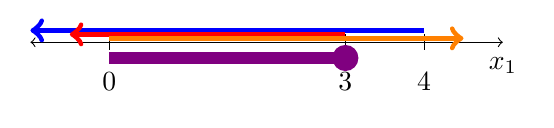
\begin{tikzpicture}
  \draw [<->] (-1, 0) to (5, 0);
  \foreach \x in {0, 3, 4}
  {
    \draw (\x, .1) to (\x, -.1);
    \node at (\x, -.5) {\x};
  }
  \node at (5, -.3) {$x_1$};

  \draw [color=blue, line width=2pt, <-] (-1, .15) to (4, .15);
  \draw [color=red, line width=2pt, <-] (-.5, .10) to (3, .10);
  \draw [color=orange, line width=2pt, ->] (0, .05) to (4.5, .05);
  \draw [color=violet, line width=4pt] (0, -.2) to (3, -.2) node [circle,fill] {};

\end{tikzpicture}
\end{center}
\begin{itemize}
  \item \textcolor{violet}{feasible region} $=$ intersection of all arrows $=$ is line segment $[0, 3]$
  \item solution
  
\begin{tikzpicture}
    \node [circle, fill, color=violet] at (0, 0) {};
  \end{tikzpicture}
   is $x_1=3$
  \item optimal objective function value is $2x_1=2(3)=6$
\end{itemize}
\end{frame}

\begin{frame} \frametitle{1D Unbounded}
  maximize $2 x_1$ \\
  subject to
  \begin{eqnarray*}
    \textcolor{blue}{-x_1} &\textcolor{blue}{\leq}& \textcolor{blue}{2} \\
    \textcolor{red}{-x_1} &\textcolor{red}{\leq}& \textcolor{red}{-1} \\
    \textcolor{orange}{x_1} &\textcolor{orange}{\geq}& \textcolor{orange}{0}
  \end{eqnarray*}

  \begin{center}
  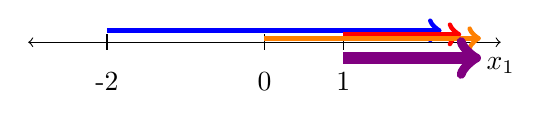
\begin{tikzpicture}
    \draw [<->] (-3, 0) to (3, 0);
    \foreach \x in {-2, 0, 1}
    {
      \draw (\x, .1) to (\x, -.1);
      \node at (\x, -.5) {\x};
    }
    \node at (3, -.3) {$x_1$};

    \draw [color=blue, line width=2pt, ->] (-2, .15) to (2.25, .15);
    \draw [color=red, line width=2pt, ->] (1, .10) to (2.5, .10);
    \draw [color=orange, line width=2pt, ->] (0, .05) to (2.75, .05);
    \draw [color=violet, line width=4pt, ->] (1, -.2) to (2.75, -.2);

  \end{tikzpicture}
  \end{center}
  \begin{itemize}
    \item \textcolor{violet}{feasible region} $=$ intersection of all arrows
      $=$ open interval $[1, +\infty)$
    \item solution is undefined
    \item optimal objective function value is $2x_1=2(\infty)=\infty$
  \end{itemize}

\end{frame}

\begin{frame} \frametitle{1D Infeasible}
  maximize $2 x_1$ \\
  subject to
  \begin{eqnarray*}
    \textcolor{blue}{x_1} &\textcolor{blue}{\leq}& \textcolor{blue}{1} \\
    \textcolor{red}{-x_1} &\textcolor{red}{\leq}& \textcolor{red}{-3} \\
    \textcolor{orange}{x_1} &\textcolor{orange}{\geq}& \textcolor{orange}{0}
  \end{eqnarray*}

  \begin{center}
  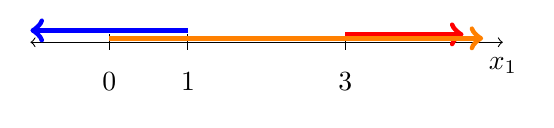
\begin{tikzpicture}
    \draw [<->] (-1, 0) to (5, 0);
    \foreach \x in {0, 1, 3}
    {
      \draw (\x, .1) to (\x, -.1);
      \node at (\x, -.5) {\x};
    }
    \node at (5, -.3) {$x_1$};

    \draw [color=blue, line width=2pt, <-] (-1, .15) to (1, .15);
    \draw [color=red, line width=2pt, ->] (3, .10) to (4.5, .10);
    \draw [color=orange, line width=2pt, ->] (0, .05) to (4.75, .05);

  \end{tikzpicture}
  \end{center}
  \begin{itemize}
    \item \textcolor{violet}{feasible region} $=$ intersection of all arrows
      $= \emptyset$
    \item solution is undefined
    \item cannot evaluate objective function
  \end{itemize}

\end{frame}

\begin{frame} \frametitle{2D Solution}
  maximize $x_2$ \\
  subject to
  \begin{eqnarray*}
    \textcolor{blue}{\frac{1}{4} x_1 + x_2} &\textcolor{blue}{\leq}& \textcolor{blue}{2} \\
    \textcolor{red}{-\frac{4}{5} x_1 + x_2} &\textcolor{red}{\leq}& \textcolor{red}{\frac{1}{2}} \\
    \textcolor{orange}{x_1, x_2} &\textcolor{orange}{\geq}& \textcolor{orange}{0}
  \end{eqnarray*}
\end{frame}

\begin{frame} \frametitle{Sidebar: Math Definition of a Line}
  \begin{itemize}
    \item recall
    \begin{itemize}
    \item slope-intercept form $y=mx+b$
    \item 2D LP constraint is $c_1 x_1 + c_2 x_2 \leq b$
  \end{itemize}
  \item substitute $x_1=x, x_2=y$, rearrange to slope-intercept:
    \begin{eqnarray*}
      c_1 x_1 + c_2 x_2 &\leq& b \\
      c_1 (x) + c_2 (y) &\leq& b \\
      -(c_1 x) & & -(c_1 x) \\
      c_2 y &\leq& -c_1 x + b
    \end{eqnarray*}
    if $c_2 >0$ then
    \[ y \leq -\frac{c_1}{c_2}x + \frac{b}{c_2} \]
    else, $c_2<0,$ dividing by $c_2$ flips $\leq$ to $\geq$, and
    \[ y \geq -\frac{c_1}{c_2}x + \frac{b}{c_2} \]
  \end{itemize}
\end{frame}

\begin{frame} \frametitle{2D Solution}
  \begin{columns}
    \begin{column}{0.4 \textwidth}
  maximize $x_2$ \\
  subject to
  \begin{eqnarray*}
    \textcolor{blue}{\frac{1}{4} x_1 + x_2} &\textcolor{blue}{\leq}& \textcolor{blue}{2} \\
    \textcolor{red}{-\frac{4}{5} x_1 + x_2} &\textcolor{red}{\leq}& \textcolor{red}{\frac{1}{2}} \\
    \textcolor{orange}{x_1, x_2} &\textcolor{orange}{\geq}& \textcolor{orange}{0}
  \end{eqnarray*}
  \begin{itemize}
    \item \textcolor{violet}{feasible region} is intersection of halfspaces
     $\Leftrightarrow$ polygon
    \item optimal solution is intersection of lines
      at $x_1 \approx 1.43, x_2 \approx 1.64$
  \end{itemize}
  \end{column}
  \begin{column}{0.6 \textwidth}
    \begin{center}
  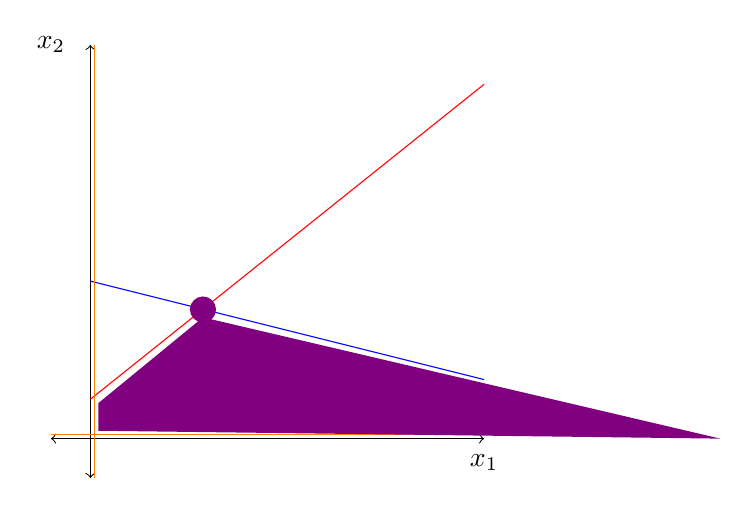
\begin{tikzpicture}
    \draw [<->] (-.5, 0) to (5, 0);
    \node at (5, -.3) {$x_1$};

    \draw [<->] (0, -.5) to (0, 5);
    \node at (-.5, 5) {$x_2$};

    \draw [color=blue] (0, 2) to (5, .75);
    \draw [color=red] (0, .5) to (5, 4.5);
    \draw [color=orange] (.05, -.5) to (.05, 5);
    \draw [color=orange] (-.5, .05) to (5, .05);

    \fill [fill=violet] (.1, .1) -- (.1, .45) -- (1.43, 1.54) -- (8, 0);
    \node [circle, fill, color=violet] at (1.43, 1.64) {};

  \end{tikzpicture}
  \end{center}
\end{column}
\end{columns}
\end{frame}

\begin{frame} \frametitle{2D Unbounded}
  \begin{columns}
    \begin{column}{0.4 \textwidth}
  maximize $x_2$ \\
  subject to
  \begin{eqnarray*}
    %\textcolor{blue}{-\frac{1}{4} x_1 + x_2} &\textcolor{blue}{\leq}& \textcolor{blue}{2} \\
    \textcolor{red}{-\frac{4}{5} x_1 + x_2} &\textcolor{red}{\leq}& \textcolor{red}{\frac{1}{2}} \\
    \textcolor{orange}{x_1, x_2} &\textcolor{orange}{\geq}& \textcolor{orange}{0}
  \end{eqnarray*}
  \begin{itemize}
    \item \textcolor{violet}{feasible region} is intersection of halfspaces
     $\Leftrightarrow$ some polygon sides, one infinite side
    \item optimal solution undefined
  \end{itemize}
  \end{column}
  \begin{column}{0.6 \textwidth}
    \begin{center}
  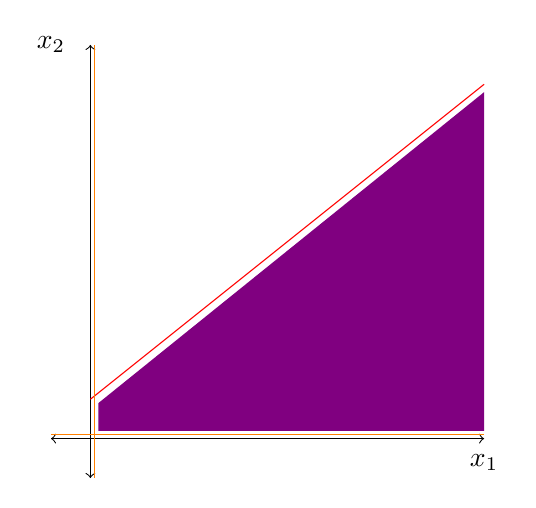
\begin{tikzpicture}
    \draw [<->] (-.5, 0) to (5, 0);
    \node at (5, -.3) {$x_1$};

    \draw [<->] (0, -.5) to (0, 5);
    \node at (-.5, 5) {$x_2$};

    %\draw [color=blue] (0, 2) to (5, .75);
    \draw [color=red] (0, .5) to (5, 4.5);
    \draw [color=orange] (.05, -.5) to (.05, 5);
    \draw [color=orange] (-.5, .05) to (5, .05);

    \fill [fill=violet] (.1, .1) -- (.1, .45) -- (5, 4.4) -- (5, .1);

  \end{tikzpicture}
  \end{center}
\end{column}
\end{columns}
\end{frame}

\begin{frame} \frametitle{2D Infeasible}
  \begin{columns}
    \begin{column}{0.4 \textwidth}
  maximize $x_2$ \\
  subject to
  \begin{eqnarray*}
    \textcolor{blue}{-x_1 + x_2} &\textcolor{blue}{\leq}& \textcolor{blue}{.25} \\
    \textcolor{red}{x_1 - x_2} &\textcolor{red}{\leq}& \textcolor{red}{2} \\
    \textcolor{orange}{x_1, x_2} &\textcolor{orange}{\geq}& \textcolor{orange}{0}
  \end{eqnarray*}
  \begin{itemize}
    \item \textcolor{violet}{feasible region} is intersection of halfspaces
     $\Leftrightarrow$ empty set
    \item optimal solution undefined
  \end{itemize}
  \end{column}
  \begin{column}{0.6 \textwidth}
    \begin{center}
  \begin{tikzpicture}
    \draw [<->] (-.5, 0) to (5, 0);
    \node at (5, -.3) {$x_1$};

    \draw [<->] (0, -.5) to (0, 5);
    \node at (-.5, 5) {$x_2$};

    \draw [color=blue] (0, .25) to (5, 5.25);
    \draw [color=red] (0, 2) to (3, 5.25);
    \draw [color=orange] (.05, -.5) to (.05, 5);
    \draw [color=orange] (-.5, .05) to (5, .05);

  \end{tikzpicture}
  \end{center}
\end{column}
\end{columns}
\end{frame}

\begin{frame} \frametitle{Slack Form}
\emph{duality:} the simplex algorithm views one LP in two ways,
\begin{enumerate}
  \item standard form
  \item \emph{slack form}
\end{enumerate}
\begin{itemize}
  \item standard form: constraint says l.h.s $\leq$ r.h.s.
  \item $\Rightarrow$ the difference or ``slack'' between l.h.s. and r.h.s.
    is $\geq 0$
  \item \emph{slack form:} constraint says l.h.s. $+$ slack $=$ r.h.s.
  \item increasing objective $=$ decreasing slack
  \item introduce one new \emph{basic variable} to represent slack in each constraint
  \item (pre-existing variables are \emph{nonbasic})
  \item $z$ = value of objective function
  \item don't bother writing ``maximize'' or ``subject to''
\end{itemize}
\end{frame}

\begin{frame} \frametitle{Standard versus Slack Form}
\begin{columns}
\begin{column}{.5\textwidth}
  maximize $x_1 + 2x_2 - \frac{1}{2} x_3$ \\
  subject to
  \begin{eqnarray*}
    \frac{1}{3} x_1 + x_3 &\leq& 5 \\
    x_1 + x_2 + x_3 &\leq& 100 \\
    x_1 - x_2 &\leq& -3 \\
    x_1, x_2, x_3 &\geq& 0
  \end{eqnarray*}
\end{column}
\begin{column}{.5\textwidth}
  \begin{eqnarray*}
    z &=& x_1 + 2x_2 - \frac{1}{2} x_3 \\
    x_4 &=& 5 - \frac{1}{3} x_1 - x_3 \\
    x_5 &=& 100 - x_1 - x_2 - x_3 \\
    x_6 &=& -3 -x_1 + x_2 \\
    & & x_1, x_2, x_3, x_4, x_5, x_6 \geq 0
  \end{eqnarray*}
  basic var's: $x_4, x_5, x_6$ \\
  nonbasic var's: $x_1, x_2, x_3$
\end{column}
\end{columns}
\end{frame}

\begin{frame} \frametitle{High-Level Simplex Algorithm}
  \begin{itemize}
    \item convert standard form LP to slack form
    \item find a feasible (probably non-optimal) initial solution
    \begin{itemize}
      \item if this does not exist, return ``infeasible''
    \end{itemize}
    \item repeat:
    \begin{itemize}
      \item choose a nonbasic variable $x_i$ with positive coefficient in objective
        function (increasing $x_i$ increases $z$)
        \begin{itemize}
          \item if no such $x_i$ exists, return solution (it's optimal)
        \end{itemize}
      \item increase $x_i$ until some basic variable $x_j$ is decreased to zero
        (``tighten'' the slack until we're up against a constraint)
        \begin{itemize}
          \item if none exists, return ``unbounded''
        \end{itemize}
      \item swap roles: rewrite slack form with $x_i$ as basic variable and
        $x_j$ as nonbasic variable
    \end{itemize}
  \end{itemize}
  (for further details, see CLRS section 29.3)
\end{frame}

\begin{frame} \frametitle{Geometric Intuition}
\begin{itemize}
  \item a solution is a point in $n$-dimensional space
  \item intuitively, initial solution is at the origin where $x_1, \ldots, x_n = 0$
  \item (for further details, see CLRS section 29.5)
  \item each iteration ``reels in'' the solution to hug the intersection between
    two constraints
  \item continues until we either
  \begin{enumerate}
    \item go ``off the map'' and know the LP is infeasible; or
    \item cannot improve any further $\Rightarrow$ found optimal solution
  \end{enumerate}
  \item each step moves us along the border of a \emph{simplex}
  \item simplex: $n$-dimensional generalization of a triangle; line segment,
    2D triangle, 3D pyramid (tetrahedron), etc.
\end{itemize}
\end{frame}

\begin{frame} \frametitle{Geometric Intuition}
\begin{center}
  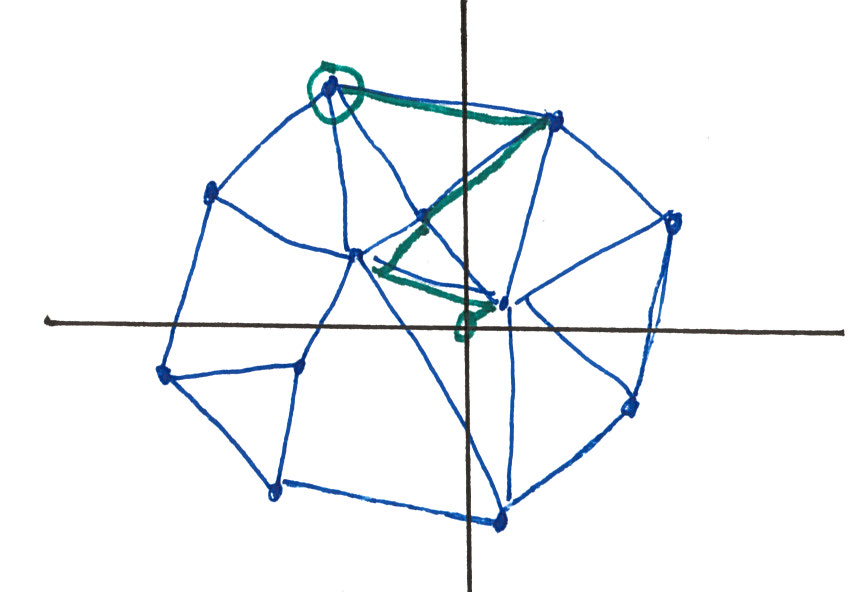
\includegraphics[width=2in]{simplex-solution.png}
  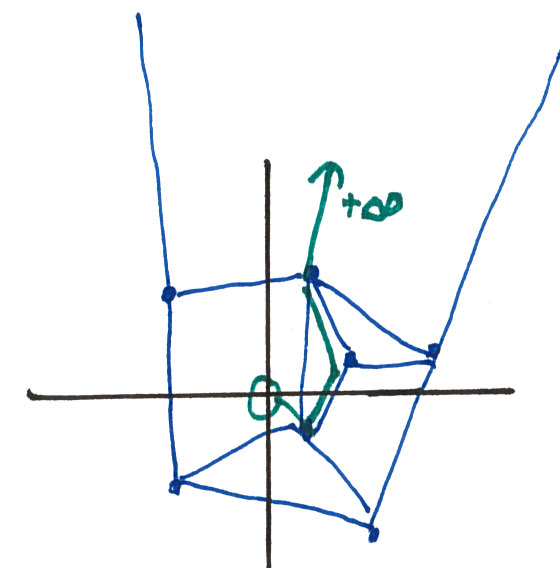
\includegraphics[width=2in]{simplex-unbounded.png}
\end{center}
\end{frame}

\begin{frame} \frametitle{Analysis}
  \begin{itemize}
    \item in LP's formulated to solve practical problems, usually
    \begin{itemize}
      \item each of the $m$ halfspaces intersects $O(m)$ other
        halfspaces
      \item $\Rightarrow O(m^2)$ intersection points in the feasible region
      \item $\Rightarrow$ simplex iterates $O(m^2)$ times
      \item each iteration involves evaluating $n$-dimension obj. function
      \item $\Rightarrow O(m^2 n)$ worst-case time
      \item order-3 polynomial, same as max-flow
      \item often faster b/c each step can ``jump'' pretty far
    \end{itemize}
    \item \textbf{however,} $\exists$ feasible LP's that force simplex to take
      $\Omega(2^m)$ time
    \item \emph{Klee-Minty cube:} $\forall d$, has $n=d$ variables, $n=d$ constraints,
      $2^d$ vertices, simplex is ``tricked'' into visiting all vertices
    \item this is a rare example of worst-case asymptotic analysis being misleading
    \end{itemize}
\end{frame}

\begin{frame} \frametitle{Klee-Minty Cube}
\begin{center}
  Klee-Minty Cube in 3D:

  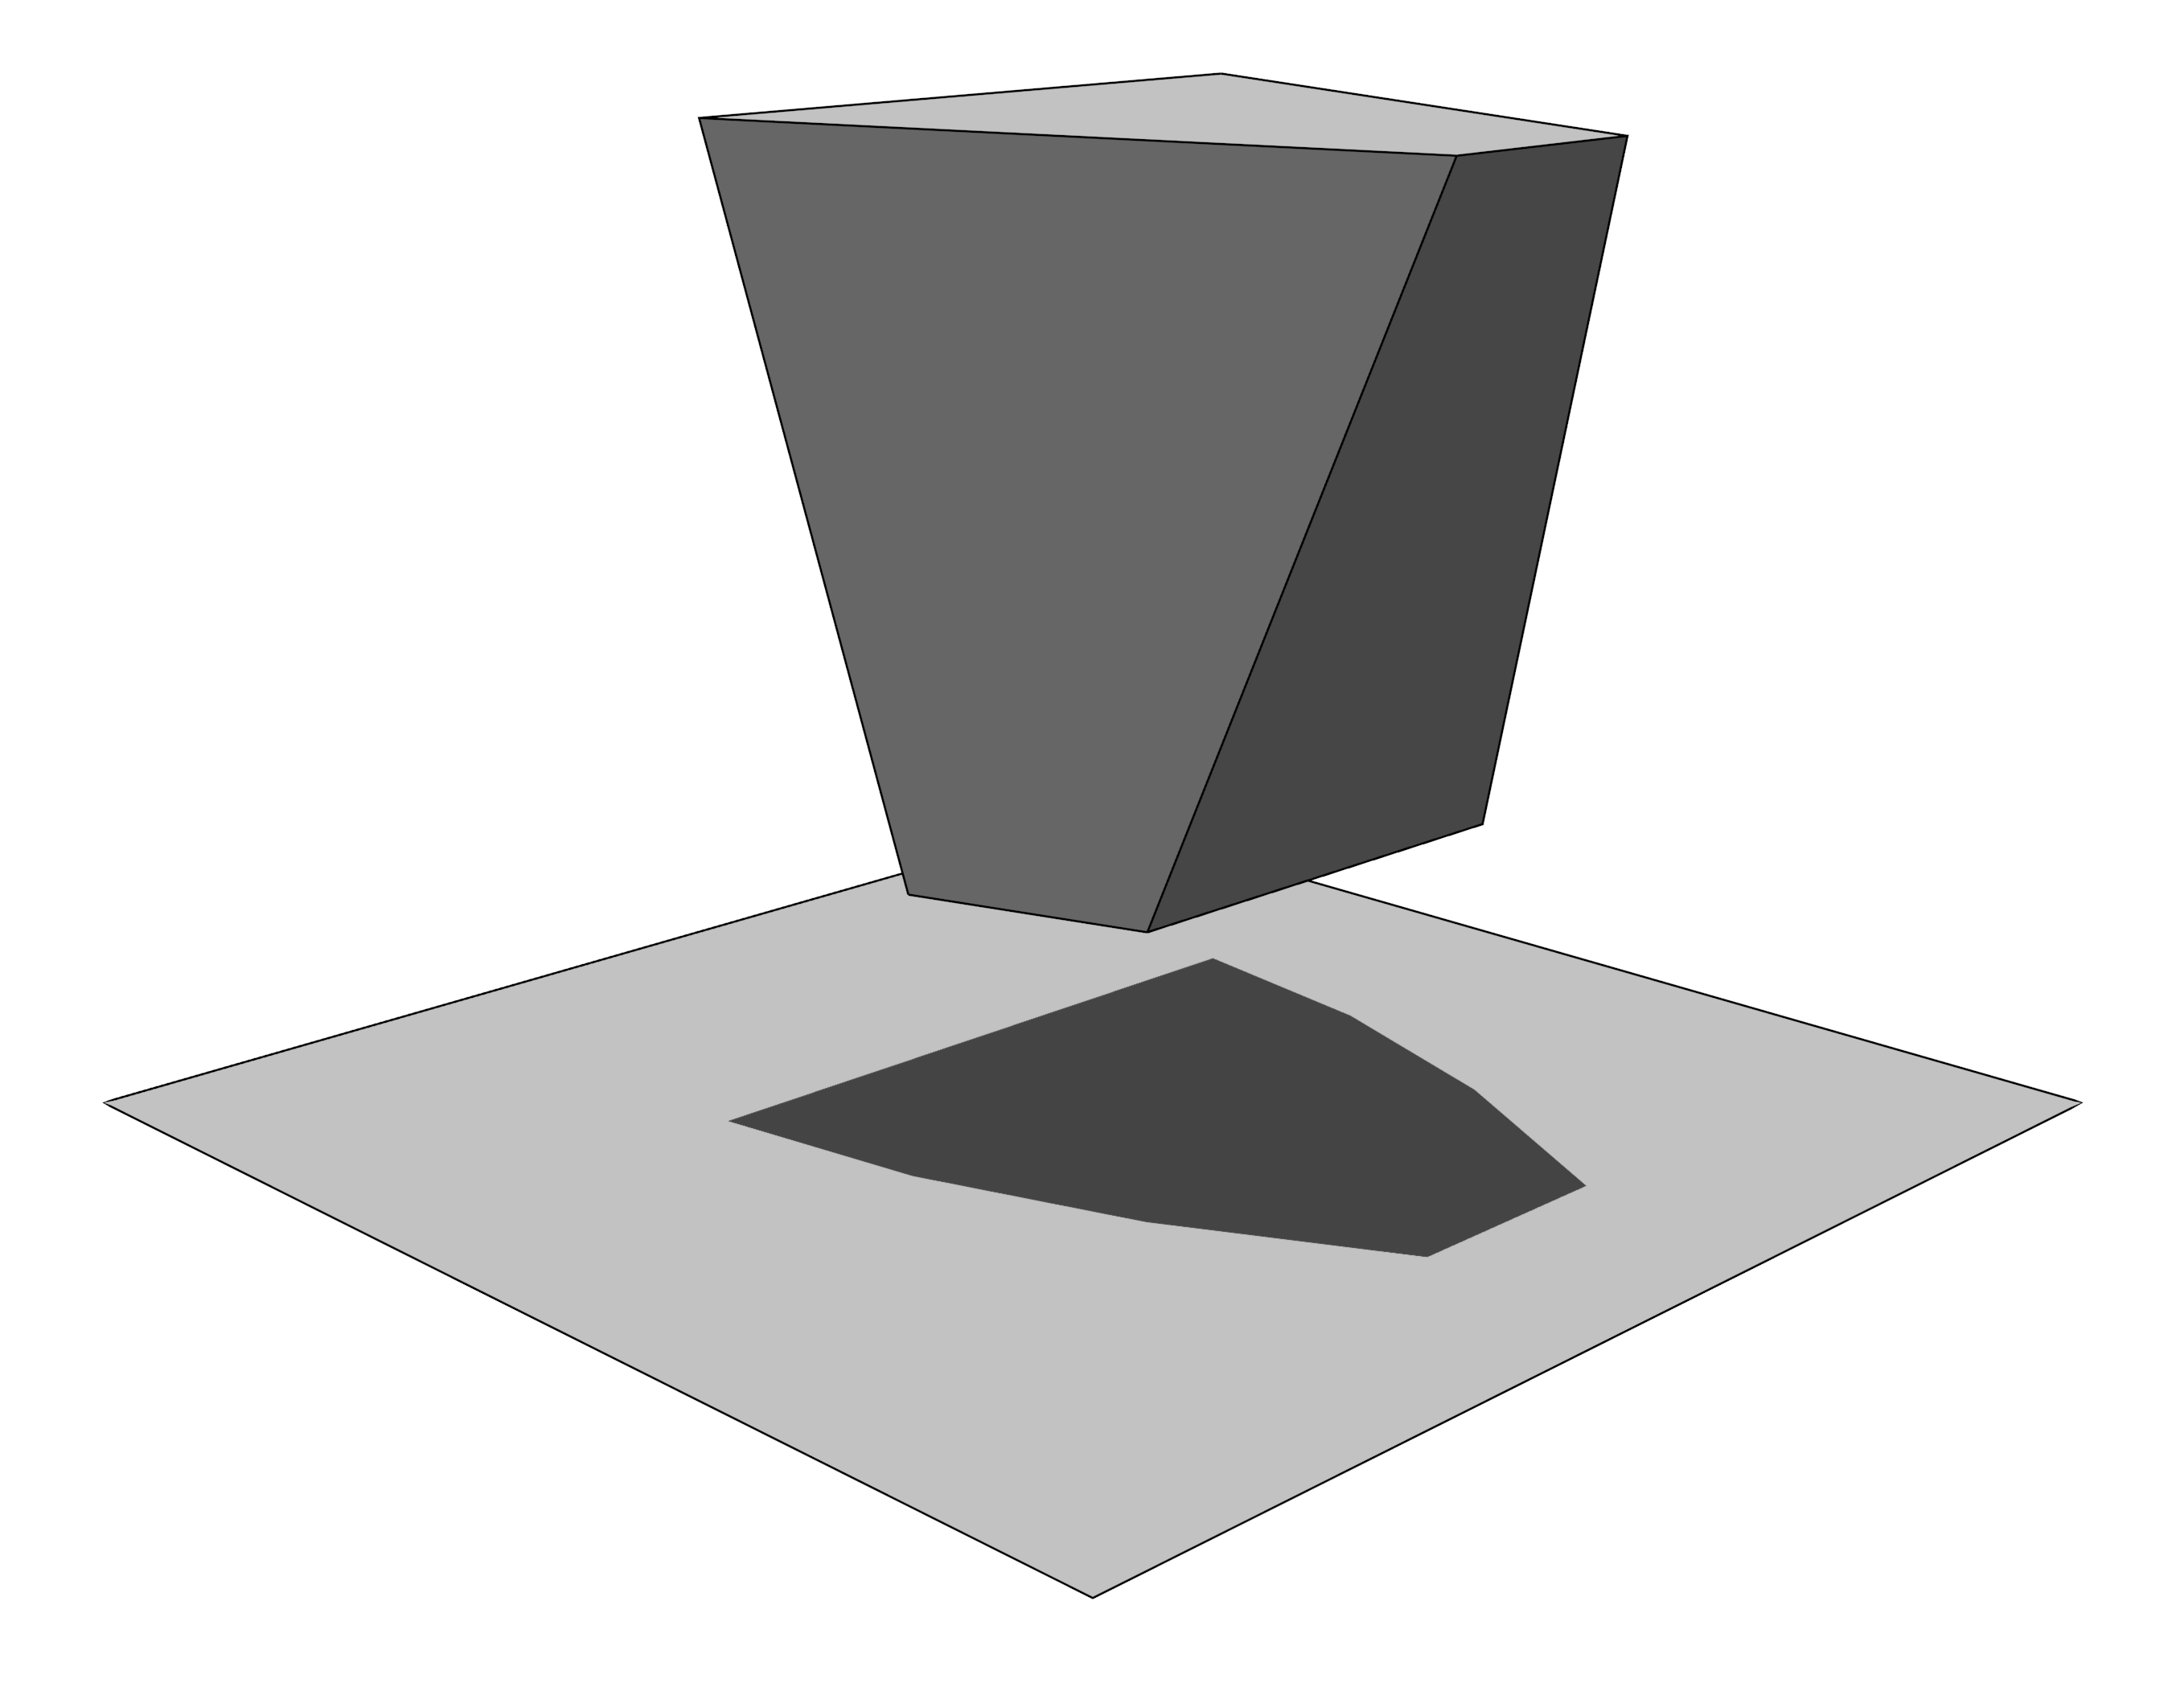
\includegraphics[scale=.07]{Klee-Minty-cube-for-shadow-vertex-pivot-rule.png}

  {\tiny
  (image credit: Sophie Huiberts, CC-BY 4.0, \url{https://commons.wikimedia.org/wiki/File:Klee-Minty-cube-for-shadow-vertex-pivot-rule.png})
  }
\end{center}
\end{frame}

\begin{frame} \frametitle{Summary}
  \begin{itemize}
    \item for a standard-form LP with $n$ variables and $m$ constraints...
    \item simplex algorithm is fast in practice, technically takes $O(2^m)$
      worst-case time
    \item Khachiyan's \emph{ellipsoid algorithm} takes $O(n^4 W)$ time
      \begin{itemize}
        \item seminal result, proved that sub-exponential algorithms are possible
      \end{itemize}
    \item now have faster pseudopolynomial algorithms, e.g Vaidya's alg.
      takes $O((n+m)^{1.5} nW )$ time
    \item open questions:
    \begin{itemize}
      \item Is there a strongly-polynomial algorithm, or is
      $LP$ $NP$-complete?
      \item Is there an algorithm that has \textbf{both}
      simplex' practical speed \textbf{and} provable pseudonomial runtime?
    \end{itemize}
  \end{itemize}
\end{frame}

\end{document}
